\chapter{Application Implementation and \\ Documentation}

Nei capitoli precedenti sono state presentate le features che devono essere implementate per il corretto funzionamento dell'applicazione Sistema Monitoraggio Ambientale nel caso in cui dovesse essere utilizzata da un utente di tipo Amministratore.
L'applicazione è stata sviluppata con \texttt{NodeJS} e \texttt{Bootstrap}. Per la gestione dei dati abbiamo utilizzato \texttt{MongoDB}.

\section{Project Structure}

Nella figura \ref{fig:projectStructure} possiamo vedere la struttura del progetto.
Esso è composto da una cartella api per la gestione delle API locali, una cartella css che contiene un file di stile, una cartella images che contiene tutte le immagini utilizzate nel progetto, una cartella js che raggruppa tutti i file javascript e infine una cartella ui che contiene le le pagine html. In fondo si può vedere anche la pagina html principale dell'applicazione e il file README.md utilizzato da github per fornire una descrizione del progetto contenuto nella repository e come eseguirlo correttamente.

\begin{figure}[ht]
    \centering
    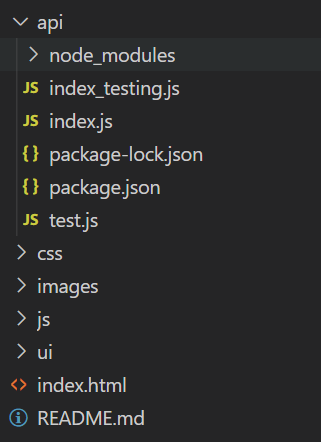
\includegraphics[scale=1]{Img/ProjectStructure.png}
    \caption{Struttura del progetto}
    \label{fig:projectStructure}
\end{figure}

\section{Project Dependencies}
I seguenti moduli Node sono stati utilizzati ed aggiunti al file \texttt{package.json}:
\begin{itemize}
    \item \texttt{Express}
    \item \texttt{Body-Parser}
    \item \texttt{Cors}
    \item \texttt{MongoDB}
    \item \texttt{Swagger-jsDoc}
    \item \texttt{Swagger-ui-Express}
    \item \texttt{sweetalert2}
\end{itemize}
\newpage
Inoltre sono stati utilizzati dei moduli per sviluppo:
\begin{itemize}
    \item \texttt{supertest}
    \item \texttt{tap-spec}
    \item \texttt{tap}
\end{itemize}

In aggiunta alle \textit{dependencies} presentate, sono stati utilizzati anche \texttt{Bootstrap}, \texttt{jQuery}, \texttt{MapBox} e \texttt{Google Charts} come script \texttt{HTML}.

\section{Project Data or DB}
Per la gestione dei dati necessari al corretto funzionamento dell'applicativo abbiamo definito 6 strutture dati come illustrato in Figura \ref{fig:DB_Structure}. Le suddette sono \texttt{"Fauna"}, \texttt{"Flora"}, \texttt{"Parco"}, \texttt{"SensoreGPS"}, \texttt{"StoricoFauna"}, \texttt{"RischioAmbientale"}.

\begin{figure}[ht]
    \centering
    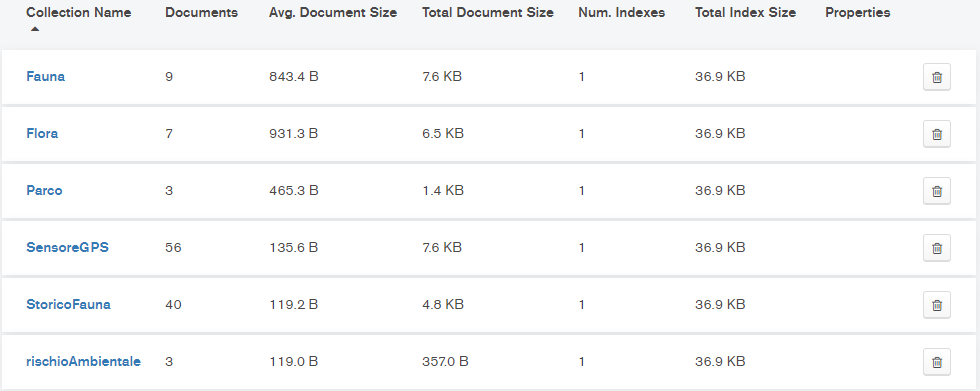
\includegraphics[scale=0.6]{Img/CollectionsMongoDB.png}
    \caption{Collezione dati utilizzati dall'applicazione}
    \label{fig:DB_Structure}
\end{figure}

\newpage
Per rappresentare le seguenti strutture dati abbiamo definito i seguenti tipi di dati (Vedi figure da \ref{fig:fauna} a \ref{fig:rischio}).

\begin{multicols}{2}
    \begin{Figure}
        \centering
        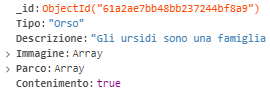
\includegraphics{Img/FaunaType.png}
        \captionof{figure}{Tipo di dato \texttt{"Fauna"}}
        \label{fig:fauna}
    \end{Figure}
    
    \begin{Figure}
        \centering
        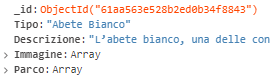
\includegraphics{Img/FloraType.png}
        \captionof{figure}{Tipo di dato \texttt{"Flora"}}
        \label{fig:flora}
    \end{Figure}
    
    \begin{Figure}
        \centering
        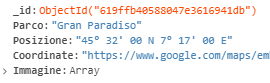
\includegraphics{Img/ParcoType.png}
        \captionof{figure}{Tipo di dato \texttt{"Parco"}}
        \label{fig:parco}
    \end{Figure}
    
    \begin{Figure}
        \centering
        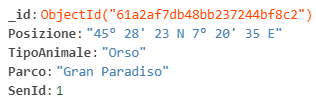
\includegraphics{Img/SensoreType.png}
        \captionof{figure}{Tipo di dato \texttt{"SensoreGPS"}}
        \label{fig:sensore}
    \end{Figure}
    
    \begin{Figure}
        \centering
        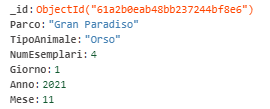
\includegraphics{Img/StoricoType.png}
        \captionof{figure}{Tipo di dato \texttt{"StoricoFauna"}}
        \label{fig:storico}
    \end{Figure}
    
    \begin{Figure}
        \centering
        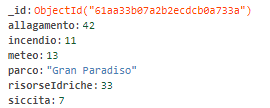
\includegraphics{Img/RischioType.png}
        \captionof{figure}{Tipo di dato \texttt{"rischioAmbientale"}}
        \label{fig:rischio}
    \end{Figure}
\end{multicols}

\newpage
\section{Project APIs}


\subsection{Elenco informazioni di un animale}
Utilizzando questa API l'applicativo può ottenere le informazioni inerenti ad un singolo animale contenuto al momento della chiamata nel sistema. L'API mediante il metodo \texttt{find(\{\})} ritorna il singolo animale inserito come parametro nella funzione. In caso venga rilevato un errore, esso verrà stampato a console.

\begin{figure}[ht]
    \centering
    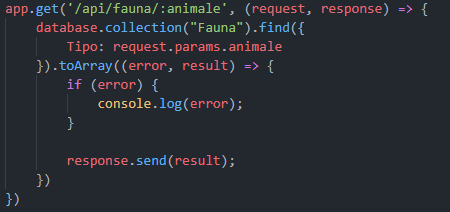
\includegraphics{Img/getFaunaByAnimal.png}
    \label{fig:get_fauna_animale}
\end{figure}

\subsection{Aggiornamento rischio ambientale in tempo reale}
La seguente API permette all'applicazione di simulare la ricezione ed inserimento nel database dei dati elaborati dal "Sistema Di Calcolo Probabilistico" (nominato molteplici volte nei documenti precedenti).

Con il metodo \texttt{updateOne(\{\},\{\})}, il sistema è in grado di modificare i valori di rischio di un parco in modo tale che le variazioni non siamo troppo elevate.

\begin{figure}[ht]
    \centering
    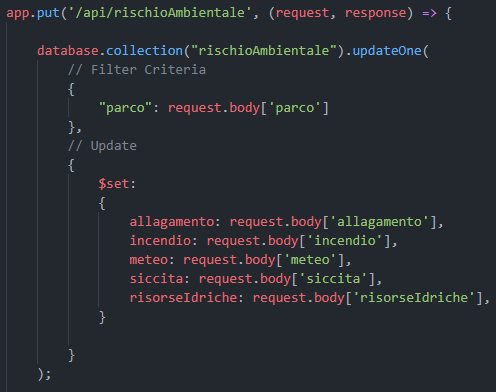
\includegraphics{Img/putRischio.png}
    \label{put_rischio}
\end{figure}

\newpage

\subsection{Aggiunta di un sensore}
Questa API viene utilizzata ogniqualvolta si desidera inserire un nuovo sensore nel sistema. 

Permette di creare un nuovo oggetto di tipo \texttt{SensoreGPS} composto da \texttt{Posizione}, \texttt{TipoAnimale}, \texttt{Parco} e \texttt{SenId} inviati come body della richiesta. Nel caso di avvenuto inserimento, viene visualizzato a console un messaggio di conferma, in caso contrario viene stampato un messaggio di errore.

\begin{figure}[ht]
    \centering
    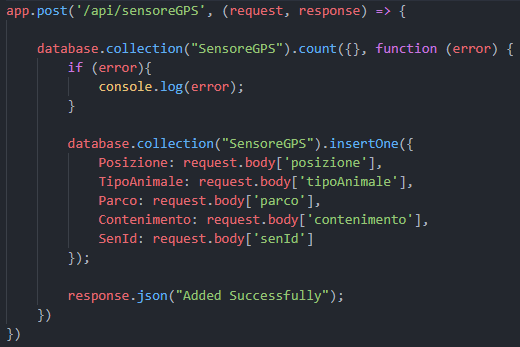
\includegraphics{Img/postSensore.png}
    \label{fig:post_sensore}
\end{figure}

\subsection{Rimozione di un sensore}
La seguente API permette all'applicazione di rimuovere un sensore dal sistema. Essa prende come input l'ID del sensore da eliminare e mediante il metodo \texttt{deleteOne(\{\})} elimina il sensore desiderato. In caso di corretta rimozione, viene visualizzato a console un messaggio di conferma.

\begin{figure}[ht]
    \centering
    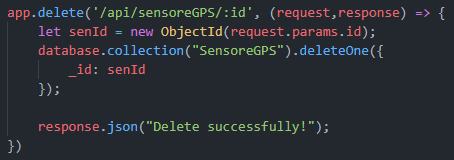
\includegraphics{Img/deleteSensore.png}
    \label{delete_sensore}
\end{figure}


% --------------- API in più -----------------

%commento
\begin{comment}
\subsection{Storico Fauna}
L'applicazione, utilizzando questa API, è in grado di ottenere dal sistema i dati relativi allo storico della fauna al momento della chiamata di quest'ultima. Essa utilizza il metodo \texttt{find({})} per ritornare i dati. Nel caso un errore venga rilevato, esso viene visualizzato a console.

\begin{figure}[ht]
    \centering
    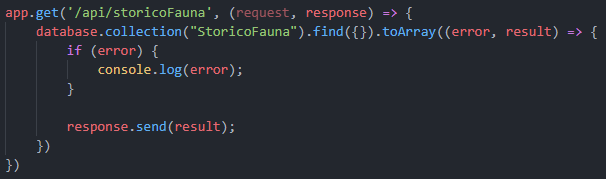
\includegraphics{Img/getStorico.png}
    \label{get_storico}
\end{figure}
\end{comment}
%commento

%commento
\begin{comment}
\subsection{Elenco fauna}
Mediante questa API l'applicazione può ottenere l'elenco degli animali contenuti al momento nel sistema. L'API ritorna l'elenco degli animali mediante il metodo \texttt{find({})} e nel caso si verifichi un errore esso verrà visualizzato a console.

\begin{figure}[ht]
    \centering
    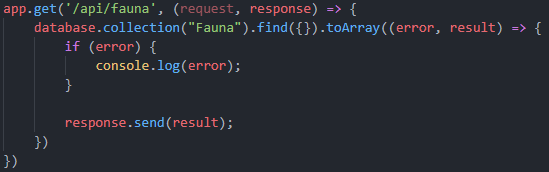
\includegraphics{Img/getFauna.png}
    \label{get_fauna}
\end{figure}
\end{comment}
%commento

%commento
\begin{comment}
\subsection{Elenco degli animali tracciati}


\begin{figure}[ht]
    \centering
    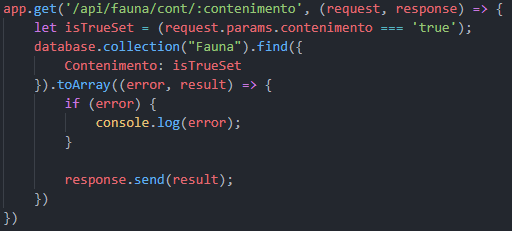
\includegraphics{Img/getFaunaByContenimento.png}
    \label{fig:get_fauna_contenimento}
\end{figure}

\subsection{Elenco flora}
Mediante questa API l'applicazione può ottenere l'elenco della fauna attualmente contenuta nel sistema. Questa API ritorna l'elenco della flora mediante il metodo \texttt{find({})} e nel caso si verifichi un errore esso verrà visualizzato a console.

\begin{figure}[ht]
    \centering
    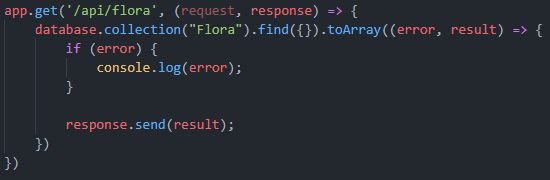
\includegraphics{Img/getFlora.png}
    \label{get_flora}
\end{figure}
\newpage
\subsection{Elenco informazioni di una pianta}

Questa API viene utilizzata dall'applicazione per ottenere i dati inerenti ad una specifica pianta. L'API ritorna la pianta selezionata utilizzando il parametro fornito in input ed utilizzandolo nel metodo \texttt{find({})}. In caso venga rilevato un errore, viene visualizzato un messaggio d'errore.
\begin{figure}[ht]
    \centering
    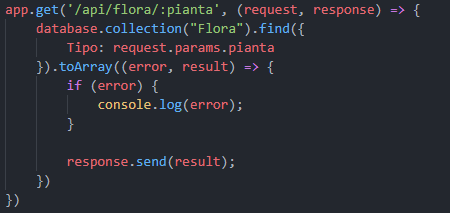
\includegraphics{Img/getFloraByPlant.png}
    \label{fig:get_flora_pianta}
\end{figure}

\subsection{Elenco parchi}
La seguente API permette all'applicazione di ottenere l'elenco dei parchi contenuti al momento all'interno del sistema ritornando il risultato del metodo \texttt{find({})}. In caso venga rilevato un errore, esso verrà stampato nella console.

\begin{figure}[ht]
    \centering
    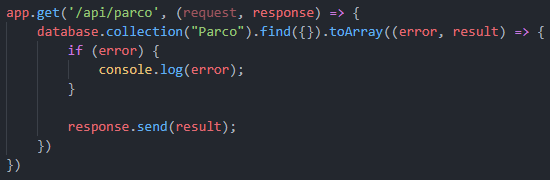
\includegraphics{Img/getParco.png}
    \label{get_parchi}
\end{figure}

\subsection{Elenco informazioni di un parco}
La seguente API permette all'applicativo di ottenere informazioni su di uno specifico parco. Essa prende in input il nome di un parco specifico ed utilizza tale argomento per selezionare, mediante il metodo \texttt{find({})}, il parco desiderato ed infine lo restituisce. In caso venga rilevato un errore, esso viene stampato in console.

\begin{figure}[ht]
    \centering
    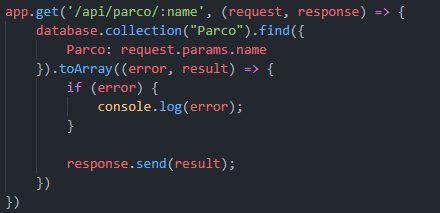
\includegraphics{Img/getParcoByName.png}
    \label{fig:get_info_parco}
\end{figure}

\newpage
\subsection{Livello Rischio}
Questa API permette all'applicazione di ottenere i livelli di rischio di tutti i parchi presenti attualmente nel sistema. L'API ritorna il risultato del metodo \texttt{find({})}, stampando a console un errore in caso esso venga rilevato.

\begin{figure}[ht]
    \centering
    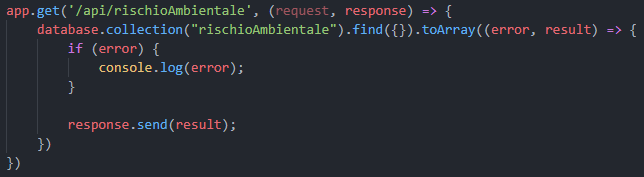
\includegraphics[scale=0.9]{Img/getRischio.png}
    \label{get_rischi}
\end{figure}

\subsection{Livello rischio di un parco}
Questa API permette all'applicazione di ottenere il livello di rischio di un parco specifico. Essa utilizza il metodo \texttt{find({})} per selezionare, utilizzando come filtro il parco inserito come argomento della funzione, i livelli di rischio del parco specifico. In caso venga rilevato un errore, esso viene visualizzato in console.

\begin{figure}[ht]
    \centering
    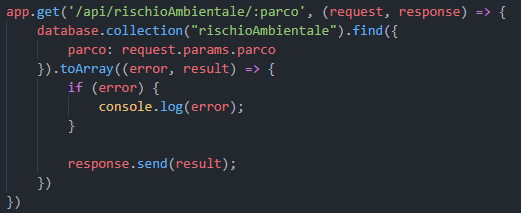
\includegraphics{Img/getRischioByParco.png}
    \label{fig:get_rischio_parco}
\end{figure}
\end{comment}
%commento

%commento
\begin{comment}
\subsection{Elenco sensori di un parco}
La seguente API permette all'applicazione di ottenere tutti i sensori GPS di un parco specifico al momento della chiamata. Ottenuto il parco come argomento della funzione, essa utilizza il metodo \texttt{find({})} per restituire tutti i sensori di quel parco specifico. In caso venga rilevato un errore, esso viene stampato a console.

\begin{figure}[ht]
    \centering
    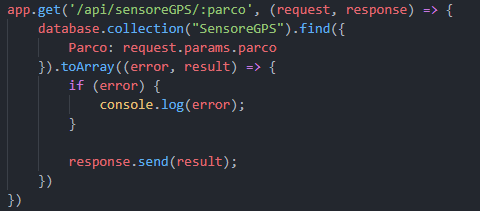
\includegraphics{Img/getSenByParco.png}
    \label{get_sensori_parco}
\end{figure}


\subsection{Elenco sensori di un animale in un parco}
La seguente API permette di ottenere i dati di uno specifico sensore in uno specifico parco presente nel sistema al momento della chiamata. Essa prende come input un animale ed un parco ed utilizzando il metodo \texttt{find({})}, seleziona il sensore correlato allo specifico animale nel parco richiesto. Un errore, in caso venga visualizzato, viene stampato in console.

\begin{figure}[ht]
    \centering
    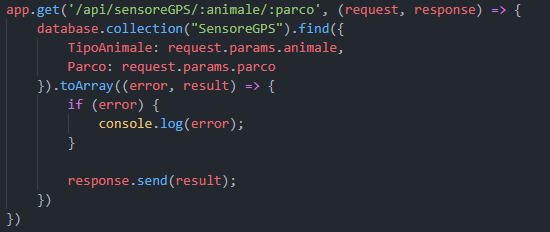
\includegraphics{Img/getSenAnimaleParco.png}
    \label{get_sensori_animale_parco}
\end{figure}
\end{comment}
%commento